\documentclass[11pt]{article}

\usepackage{tikz}
\usetikzlibrary{arrows}
\usepackage[margin=1in]{geometry}
\usepackage{listings}
\usepackage{color}
\usepackage{program}



\title{Cyberinfrastructure Foundations: Final}
\author{Matthew Le}

\begin{document}
\maketitle

1. (5 points) Discuss how cyberinfrastructure will change science and engineering research in your domain with justifications.

{\bf My research revolves around designing programming languages that allow programmers to easily develop parallel applications.  As parallel architectures evolve, the compilers and runtime systems for these languages must evolve with them.  }\\


2. (5 points)Middleware enables remote method invocation for distributed objects, so that a thread can use remote objects like local ones. Java RMI is one of them. Discuss in detail how Java RMI makes this possible. Use a diagram and discuss each component briefly.

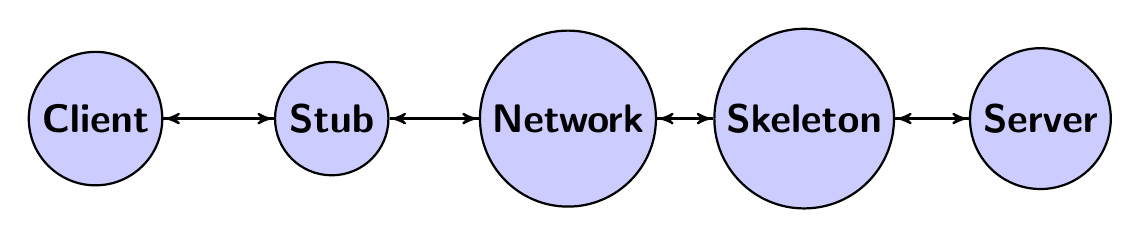
\begin{tikzpicture}[->,>=stealth',shorten >=1pt,auto,node distance=3cm,
  thick,main node/.style={circle,fill=blue!20,draw,font=\sffamily\Large\bfseries}]
  
  \node[main node] (Client){Client};
  \node[main node] (Stub)[right of=Client]{Stub};
  \node[main node] (Network)[right of=Stub]{Network};
  \node[main node] (Skeleton)[right of=Network]{Skeleton};
  \node[main node] (Server)[right of =Skeleton]{Server};
  
  \path[every node/.style={font=\sffamily\small}]
  	(Client) edge node [left]{} (Stub)
	(Stub) edge node [right]{}(Client)
	(Stub) edge node [right]{}(Network)
	(Network) edge node [right]{}(Stub)
	(Network) edge node [right]{}(Skeleton)
	(Skeleton) edge node [left]{}(Network)
	(Skeleton) edge node [right]{}(Server)
	(Server) edge node [right]{}(Skeleton)
	;
  
\end{tikzpicture} \\

3. (9 points) Answer the following questions:

1) Study MPI, and discuss five message passing functions of your choice.
{\bf
\begin{itemize}
\item MPI\_Send -- Sends a chunk of memory to another node, blocking until the message is received
\item MPI\_Recv -- Tries to receive a message from another node, blocking until the message is sent
\item MPI\_Bcast -- sends a message to all other processes in the group
\item MPI\_Gather -- collects values from a group of processes
\item MPI\_Reduce -- Folds a given operation over a set of values provided by a group of processes
\end{itemize}
}


2) AWS is Amazon's public cloud service. Take a look at its services, and discuss how it provides computing and storage services.

{\bf
Amazon AWS provides compute and storage cloud services.  The compute services form a cluster architecture, where users are able to use varying number of processors to meet the needs of their computational challenges.  
}

3) Find one grid computing service, and discuss its architecture.

5. (3 points) Write a sequential algorithm for Q4.

\begin{figure}[h]
\begin{program}
\PROC floydWarshall(G) \BODY
	n = size(G); \rcomment{Number of vertices in G}
	D = \text{new } n \; X \; n \text{ matrix}
	\FOR 
	
\END
\end{program}
\end{figure}


6. (3 points) Convert the sequential algorithm to a parallel one.

7. (5 points) Breadth-first search conducts exhaustive search that visits all of the nodes in a graph. This is why breadth-first search is a popular algorithm for problem solving. Give a sketch of the breadth-first search algorithm. Your sketch must be specific like pseudo- code.

\begin{figure}[h]

\begin{program}
\PROC bfs(G, s) \BODY

	Q = EmptyQueue;
	Q.deque(s);
	\WHILE(!Q.isEmpty()) \DO
		n = Q.deque()
		n.seen = true;
		\FOR v\; |in| \; neighbors(n)\; \DO
			Q.enque(v);
		\END
	\END
	
\END
\end{program}

\end{figure}

8. (10 points) Study what the knapsack problem is. Define the problem, and then suggest a dynamic-programming based solution.

{\bf The knapsack problem is defined as follows.  Given knapsack with total capacity $C$ and a list of $n$ items each with weight $w_i$ and value $v_i$, you need to maximize the value of the items that can fit in the knapsack without going over the maximum capacity.  This can be solved using dynamic programming by creating an array, $m$ from $1$ to $C$. We then recursively define $m$ as follows:

\[
m(w) = \begin{cases}
	0& w = 0 \\
	\max\limits_{w_i \le w}(v_i + m[w - w_i]) & otherwise
\end{cases}
\]}

9. (2 points) Compare the architecture of shared memory multiprocessor systems with that of message passing based cluster parallel systems. Also, discuss their pros and cons.

{\bf
Shared memory multiprocessor systems are those that make use of multicore processors on a single machine that all have access to the same main memory.  Cluster parallel systems on the other hand are distributed amongst multiple machines are require communication to be done via message passing rather than shared memory.  Shared memory parallel architectures more readily available in the sense that pretty much every machine available on the market these days is a shared memory parallel architecture.  Also, they are better for fine grained concurrency as synchronization is cheaper since it only requires access to memory rather than sending a message across a network.  

Cluster parallel architectures perform better on very coarse grained parallelism, where each node in the cluster needs to compute a lot of work.  Cluster machines often have a substantial amount of processing power, so are very useful for applications such as those that fit into the map reduce framework.  
}\\

10. (3 points) In the AES encryption problem, our program searches for a portion of the 256-bit key that matches a given plaintext to its ciphertext. It uses a brute-force attack which searches the entire search space. \\

(a) Is this problem a proper candidate for embarrassingly parallel computation? Explain why or why not.

{\bf Yes it is a good candidate for embarrassingly parallel processing as there are no sequential dependencies anywhere in the program.  The search space can be evenly divided amongst the processing resources without any synchronization.}\\

(b) Suppose that the most significant 192 bits of the key are already known. If the program creates 8 threads, how many encryptions does each thread need to compute if the workloads are well-balanced among the threads?

{\bf
This leaves 64 bits of the key remaining, so we must try $2^{64}$ different combinations.  If we have 8 ($2^3$) threads, then each thread must handle $\frac{2^{64}}{2^3} = 2^{61}$ different combinations.
}\\

11. (4 points) The following table shows problem size N, running time T (msec), and the number of processors K for a parallel program. Magically, the sequential program shows the same running time as the parallel program with K=1.

(a) Calculate Speedup and Eff for N=40 and K=4.

{\bf Speedup = 2.344X and Efficiency = 58.6\% (compared against K = 1)} \\

(b) What is the sequential fraction F of the total running time for K=4, N=360? Using the given data and Amdahl's law, you can calculate F easily. Your F must have six digits after the decimal point.
\begin{displaymath}
\begin{array}{rcll}
T(N, K) &=& T(N, 1) \times F + \frac{(1 - F) \times T(N, 1)}{K} \\
4896 &=& 17165 \times F + \frac{(1 - F) \times 17165}{4} \\
4896 &=& 17165 \times F + 4291.25 - 4,291.25 \times F \\
604.75 &=& 12,873.75 \times F \\
0.046975 &=& F

\end{array}
\end{displaymath}

(c) Using the value of F computed in the previous question, calculate the running time in msec when N=360 and K=6.

\begin{displaymath}
\begin{array}{rcll}
T(360, 6) &=& 0.046975 \times17165 + \frac{(1 - 0.046975) \times 17165}{6} \\
T(360, 6) &=& 806.33 + 2726.446 \\
T(360, 6) &=& 3532.78

\end{array}
\end{displaymath}

(d) Calculate N, Sizeup, and SizeupEff for K=3 and T=5000? Give the answer with two digits after the decimal point.

12. (1 point) In the Mandelbrot set problem, when we divide the problem space equally among threads, we witnessed slowdown, not speedup, with even more threads. Explain why this occurred.

{\bf The problem is a load balancing issue.  It does not take the same amount of time to compute the value of each pixel in the matrix, so threads computing the values for the center of the matrix take more time than those on the edges of the matrix.}\\

13. (1 point) How can we mitigate the slowdown problem discussed in Q 12?

{\bf This can be solved using the Master-Worker design pattern, where we maintain a global counter of the next pixel to be computed.  Each time a thread finishes computing a pixel it performs an atomic fetch and add on the global counter and processes this pixel location}

14. (10 points) Suppose that you write a cluster parallel program that multiplies two n x n square matrices A and B and produces another n x n square matrix C. Answer the following questions regarding that question:

(a) Suppose that there are p processors available. Explain how you divide matrices A and B into blocks each of which is assigned to a processor.

(b) Suppose that each process initially generates the elements of its own block. After that, what kind of message passing do we need for the matrix multiplication? Be specific on why and how.

\end{document}
















